% Created 2015-08-13 qui 03:01
\documentclass[11pt]{article}
\usepackage[latin1]{inputenc}
\usepackage[T1]{fontenc}
\usepackage{fixltx2e}
\usepackage{graphicx}
\usepackage{longtable}
\usepackage{float}
\usepackage{wrapfig}
\usepackage{rotating}
\usepackage[normalem]{ulem}
\usepackage{amsmath}
\usepackage{textcomp}
\usepackage{marvosym}
\usepackage{wasysym}
\usepackage{amssymb}
\usepackage{hyperref}
\tolerance=1000
\author{Marcelo da Mata Oliveira}
\date{\today}
\title{Lecture 1 - Experiment}
\hypersetup{
  pdfkeywords={},
  pdfsubject={},
  pdfcreator={Emacs 25.0.50.1 (Org mode 8.2.10)}}
\begin{document}

\maketitle
\tableofcontents


\section{Introduction}
\label{sec-1}
In ophthalmology there are many tests that can perform in a non invasive way. In order to do that automatically we will use a smartphone to perform a psychophysical tests.

We can control the intensity of a point in the screen of smartphone by absolute values, but we want this values in a standard measurement unit, wich is commonly used by professionals of this field.

This report will describe how we made our experiment and show some results got.

\section{Method}
\label{sec-2}
We used a device called luximetry to get measurements of a point's intensities in the screen. In order to block the light from outside, we built a small paperboard box and we painted it inside with black color to minimize possible effects light reflectance.

The point area painted in the screen was measured in 3 different sizes, with diameters of 300, 200 and 100 millimeters.

\section{Results}
\label{sec-3}
\begin{figure}[htb]
\centering
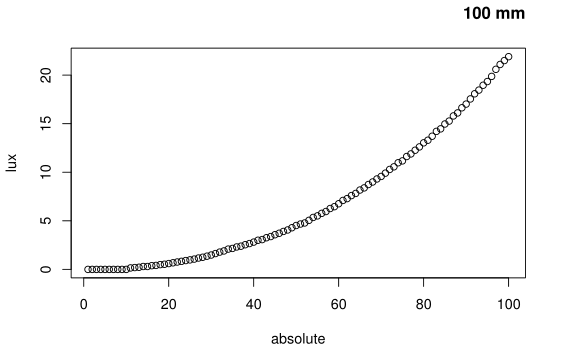
\includegraphics[width=.9\linewidth]{./m100.png}
\caption{\label{Measurements-of-differents-sizes}Relation lux x absolute}
\end{figure}
\begin{figure}[htb]
\centering
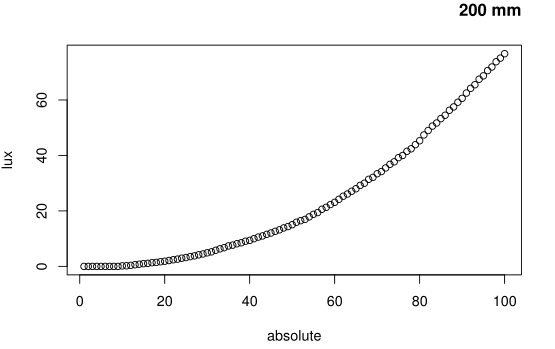
\includegraphics[width=.9\linewidth]{./m200.png}
\caption{\label{Measurements-of-differents-sizes}Relation lux x absolute}
\end{figure}
\begin{figure}[htb]
\centering
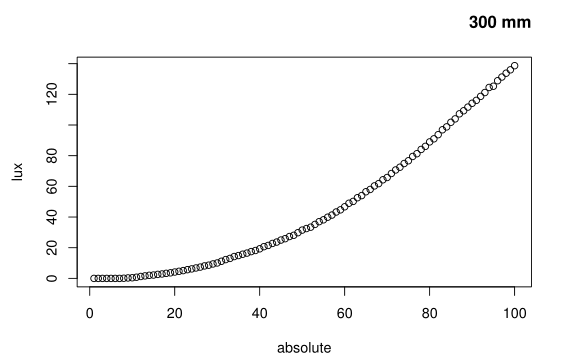
\includegraphics[width=.9\linewidth]{./m300.png}
\caption{\label{Measurements-of-differents-sizes}Relation lux x absolute}
\end{figure}
% Emacs 25.0.50.1 (Org mode 8.2.10)
\end{document}
